\documentclass[10pt,a4paper,titlepage]{article}
\usepackage[latin1]{inputenc}
\usepackage[english]{babel}
\usepackage[margin=1.2in]{geometry}
\usepackage{amsmath}
\usepackage{amsfonts}
\usepackage{amssymb}
\usepackage{makeidx}
\usepackage{graphicx}
\usepackage{float}
\usepackage[justification=centering]{caption}
\renewcommand{\labelitemi}{$\bullet$}
\author{Wim Boes \& Robbe Van Rompaey}
\title{LSTM LANGUAGE MODELING\\Experiments on training parameters}
\date{November 14, 2016}
\begin{document}

\maketitle	

\setcounter{tocdepth}{2}
\tableofcontents

\newpage

\section{Introduction}

\subsection{Setup of experiments}
\label{sec:setup}

The purpose of these experiments is to investigate the impact of the different training parameters involved when using recurrent neural networks for language modeling. To this end, the TensorFlow tutorial model of a recurrent neural network for language modeling (publicly available) is used with the Penn TreeBank dataset for training, validation and testing of the model \cite{tensorflow}.\\
\\
The TensorFlow tutorial language model consists of different parts. The input words, represented by word IDs (integers) unique to each word, are first embedded into multidimensional representations. These are then sequentially fed into a recurrent neural network that consists of layers of LSTM cells \cite{LSTM}. The outputs of this neural network are then turned into a probability vector by a softmax classifier. Each element of this vector is the probability that the next word is the word whose word ID is the index of the element in this vector.\\
\\
This language model uses the Penn TreeBank (PTB) dataset, a popular benchmark for language models \cite{PTB}. This dataset has a vocabulary of 10000 words and is split into train, validation and test sets. It is a relatively small dataset. Out-of-vocabulary words are mapped to a special $<$unk$>$-token that is also a part of the vocabulary.\\
\\
The principles and architecture of the model will be explained in more detail in the final thesis.

\subsection{Explanation of training parameters}
\label{subsec:exp}

This section contains an overview of the different training parameters that will be referenced throughout the rest of this document. These training parameters can be changed in the TensorFlow tutorial language model (Python) files. \\
\\
The parameters mentioned in this section will be explained in more detail in the final thesis.

\subsubsection{init\_scale}
	
All weights of the language model (the weights of the neurons of the neural network, the coefficients of the logistic regression used in the softmax function, etc.) are initialized uniformly in the range $[\textbf{-init\_scale},\textbf{init\_scale}]$.

\subsubsection{keep\_prob}

The used neural network uses dropout to prevent overfitting to the training data \cite{dropout}. \textbf{keep\_prob} is the probability of keeping the outputs of each layer (applied to each element of the output separately, not to the output as a whole). The kept outputs are adjusted with a correction factor to conserve the energy in the connection.

\subsubsection{num\_layers}

As mentioned in section \ref{sec:setup}, the neural network consists of layers of LSTM cells. The parameter \textbf{num\_layers} indicates how many layers are present in the model.

\subsubsection{num\_steps}
\label{subsubsec:numsteps}

The gradients used during training (by the optimization algorithms) are calculated by the backpropagation through time algorithm, in which the the recurrent neural network is unfolded and regarded as a deep network \cite{bptt}. The parameter \textbf{num\_steps} indicates the number of unfolded layers used.

\subsubsection{hidden\_size}

This parameter indicates the number of neurons in each hidden layer.

\subsubsection{embedded\_size}

As mentioned in section \ref{sec:setup}, the word IDs (integers) are transformed into multidimensional (real-valued) representations called word embeddings. The number of dimensions used is indicated by the parameter \textbf{embedded\_size}.

\subsubsection{learning\_rate}

The parameter \textbf{learning\_rate} indicates the starting learning rate of the optimization algorithm (see also section \ref{subsubsec:opt}).

\subsubsection{lr\_decay}
\label{subsubsec:decay}

As described in section \ref{subsubsec:max}, after \textbf{max\_epoch} epochs exponential learning rate decay is applied with factor \textbf{lr\_decay}.

\subsubsection{max\_epoch}
\label{subsubsec:max}

This is the number of training epochs without learning rate decay. For example, if \textbf{max\_epoch} is 4 and \textbf{max\_max\_epoch} (see section \ref{subsubsec:maxmax}) is 8, the first 4 epochs the optimizer will use the initial learning rate and the last 4 epochs learning rate decay will be applied (see section \ref{subsubsec:decay}).

\subsubsection{max\_max\_epoch}
\label{subsubsec:maxmax}

This parameter indicates the maximum number of training epochs. Early stopping is applied in the following way: if the current validation perplexity is not lower than the highest validation perplexity of the previous three epochs, training is stopped.

\subsubsection{max\_grad\_norm}

The gradients calculated by the backpropagation through time algorithm are clipped at a threshold, namely \textbf{max\_grad\_norm}, to prevent the exploding gradients problem \cite{bptt,exp}.

\subsubsection{batch\_size}

\textbf{batch\_size} is the number of training examples per batch. One training example contains \textbf{num\_steps} words (see section \ref{subsubsec:numsteps}). After each batch the parameters are updated, so that these are updated mutiple times during one epoch.

\subsubsection{optimizer}
\label{subsubsec:opt}

This parameter indicates which optimization algorithm (available in the Tensorflow package) is used to train the model (by minimizing the loss function, see section \ref{subsubsec:loss}) \cite{opt}. The possible values of \textbf{optimizer} are the following:

\begin{itemize}

	\item \textit{``GradDesc''}: gradient descent algorithm.
	\item \textit{``Adadelta''}: Adadelta algorithm.
	\item \textit{``Adagrad''}: Adagrad algorithm.
	\item \textit{``Momentum''}: Momentum algorithm, with a fixed momentum term of 0.33 (arbitrary value).
	\item \textit{``Adam''}: Adam algorithm

\end{itemize}

\noindent
For \textit{``Adadelta''}, \textit{``Adagrad''} and \textit{``Adam''}, the default hyperparameters in the TensorFlow package are chosen. 

\subsubsection{loss\_function}
\label{subsubsec:loss}

This parameter indicates which loss function is used by the optimizer (see section \ref{subsubsec:opt}). There are two options for \textbf{loss\_function}:

\begin{itemize}
	
	\item \textit{``full\_softmax''}: cross-entropy using full softmax:
	\[ \text{loss} = -\frac{1}{N} \sum_{i=1}^{N} \ln p_{target_{i}} \]
	\noindent
	with $p_{target_{i}}$ the probability indicated by the output of the language model (see section \ref{sec:setup}) on the position of the target word and N the length of the considered text piece (\textbf{num\_steps}). This corresponds to the Shannon-McMillan-Breimann approximation of the cross-entropy of the language model \cite{cross}.
	
	\item \textit{"sampled\_softmax"}: same loss function as above with some modifications. For the above loss function, for each target word the probability of every word in the vocabulary needs to be computed to obtain  the properly normalized probability $p_{target_{i}}$. For vocabularies that are large, this is impractical. Hence, this loss function samples the vocabulary (32 samples in this case) to compute an approximation of the properly normalized $p_{target_{i}}$, this speeds up training. This loss function can only be used during training, not during inference (because the probability is not properly normalized) \cite{sampled}.
	
\end{itemize}

\newpage
\section{Results and conclusions of experiments}
\label{sec:results}

This section contains the results and conclusions of the different experiments as described in section \ref{subsec:perf}. As mentioned there, the names of the subsections in this section refer to the variable parameters of the experiment. Each figure shows the different values of the variable parameters as well as the values of the fixed parameters.\\
\\
Some of the figures display the test/validation perplexity as a function of the number of training epochs. The (average-per-word) test/validation perplexity is equal to the exponential value of the average negative log probability (cross-entropy) of the target (test/validation) words:

\[ e^{-\frac{1}{N} \sum_{i=1}^{N} \ln p_{target_{i}}} \]

\noindent
Some of the tables include the training speed in function of the values of the variable parameters. This speed is expressed in words per seconds. All experiments are performed on the same machine so the training rate of the different test runs can be compared.

\subsection{Performed experiments}
\label{subsec:perf}

In this section, the list of performed experiments is given. In each experiment, one or more parameters are variable while the rest of the parameters stay fixed. The fixed parameters are based on the medium configuration of the TensorFlow tutorial model. Each network is also initialized in the same way (by setting the seed of the random initializer). The next list indicates the variable parameters of each experiment:

\begin{itemize}
	\item \textbf{learning\_rate \& lr\_decay}
	\item \textbf{init\_scale \& hidden\_size}
	\item \textbf{hidden\_size} \textbf{\&} \textbf{embedded\_size}
	\item \textbf{max\_grad\_norm}
	\item \textbf{num\_layers}
	\item \textbf{num\_steps} \textbf{\&} \textbf{batch\_size}
	\item \textbf{num\_steps}
	\item \textbf{optimizer}
	\item \textbf{loss\_function}
\end{itemize}

\noindent
The names of the subsections (one subsection for each experiment) in section \ref{sec:results} will refer to these variable parameters.

\newpage
\subsection{learning\_rate \& lr\_decay}

\begin{table}[H]
\centering
\caption{Last training, validation and test perplexities and the training speed with \textbf{learning\_rate \& lr\_decay} as variable parameters.}
\label{tab:exp1data}
\begin{tabular}{|l|l|l|l|l|l|}
\hline
{\small Name} & {\small Train PPL} & {\small Valid PPL} & {\small Test PPL} & {\small Average speed}\\ \hline
{\small learning\_rate = 0.1, lr\_decay} = 0.2           & 214.4731   & 209.3648   & 204.0305   & 5316.4381  \\ \hline
{\small learning\_rate = 0.5, lr\_decay} = 0.2           & 90.1018    & 106.3778   & 103.5632   & 5311.6258  \\ \hline
{\small learning\_rate = 1.0, lr\_decay} = 0.2           & 78.1643    & 96.0926    & 92.7933    & 5324.2165  \\ \hline
{\small learning\_rate = 0.1, lr\_decay} = 0.8           & 160.0688   & 163.6912   & 159.6735   & 5324.8893  \\ \hline
{\small learning\_rate = 0.5, lr\_decay} = 0.8           & 66.5606    & 96.0881    & 93.0609    & 5308.7686  \\ \hline
{\small learning\_rate = 1.0, lr\_decay} = 0.8           & 56.8053    & 88.9418    & 85.3886    & 5316.8231  \\ \hline
{\small learning\_rate = 0.1, lr\_decay} = 1.0           & 84.6244    & 118.6662   & 117.5150   & 5319.1841  \\ \hline
{\small learning\_rate = 0.5, lr\_decay} = 1.0           & 60.9704    & 97.5769    & 95.6626    & 5317.9425  \\ \hline
{\small learning\_rate = 1.0, lr\_decay} = 1.0           & 64.2170    & 93.3527    & 91.0134    & 5313.8851  \\ \hline
\end{tabular}
\end{table}

\begin{figure}[H]
	\begin{center}
		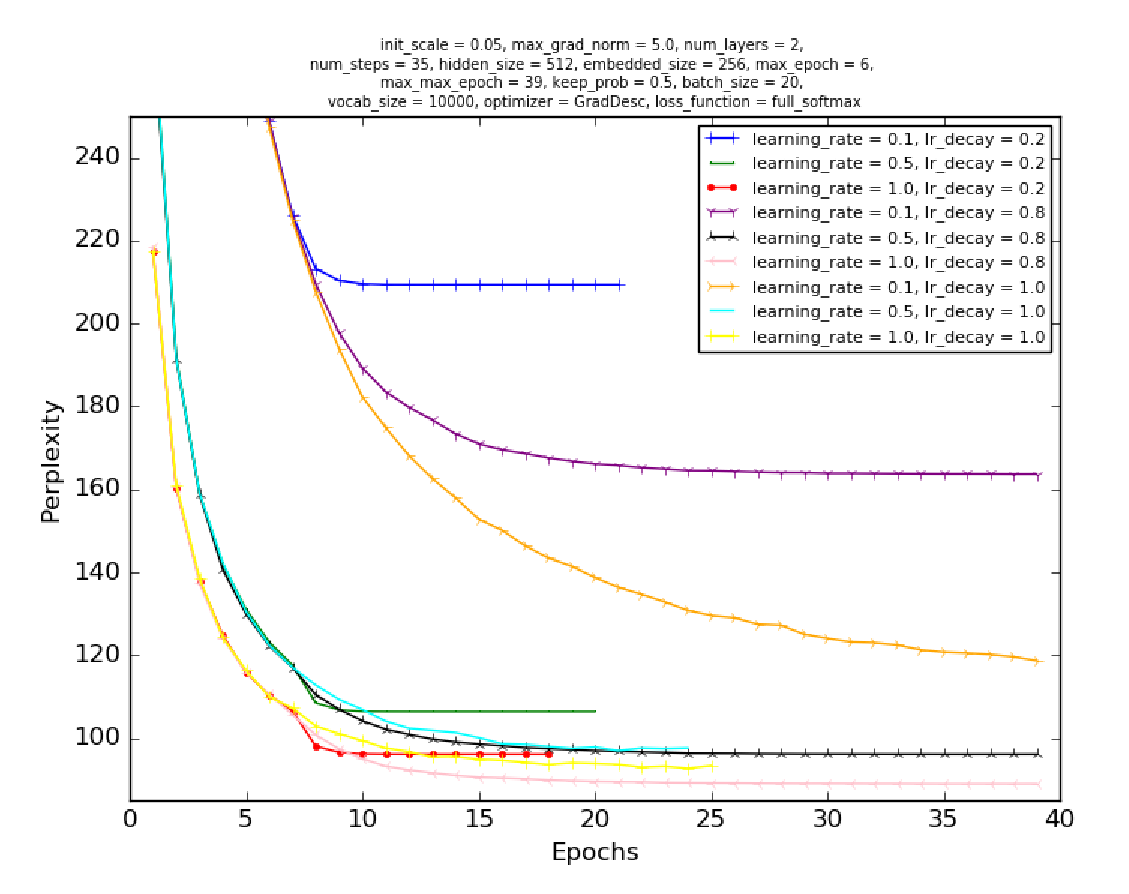
\includegraphics[width=0.85\textwidth]{Figures/learninglrdecayperf.eps}
		\caption{Convergence plot of the validation perplexity of the experiment with \textbf{learning\_rate \& lr\_decay} as variable parameters. }
		\label{fig:exp1perf}
	\end{center}	
\end{figure}

The results of this experiment are displayed in table \ref{tab:exp1data} and figure \ref{fig:exp1perf}. The most apparent conclusion of this experiment is the fact that the learning rate should not be too small. The tests with \textbf{learning\_rate} equal to 0.1 perform the worst. This is because the learning rate is too low and exponential learning rate decay is applied too early. This is clearly visible in the figure, especially when \textbf{lr\_decay} is large. The performance of the other tests are much better, in this case there seems to be a local optimum for \textbf{learning\_rate} equal to 1 and \textbf{lr\_decay} equal to 0.8.

\newpage

\subsection{init\_scale \& hidden\_size}

\begin{table}[H]
\centering
\caption{Last training, validation and test perplexities and the training speed with \textbf{init\_scale \& hidden\_size} as variable parameters.}
\label{tab:exp2data}
\begin{tabular}{|l|l|l|l|l|l|}
\hline
{\small Name} & {\small Train PPL} & {\small Valid PPL} & {\small Test PPL} & {\small Average speed}\\ \hline
{\small init\_scale = 0.005, hidden\_size = 128}         & 125.4301   & 122.0181   & 116.7535   & 11288.7535 \\ \hline
{\small init\_scale = 0.005, hidden\_size = 512}         & 58.1604    & 90.2953    & 86.3675    & 5298.5033  \\ \hline
{\small init\_scale = 0.05, hidden\_size = 128}          & 124.6025   & 120.4653   & 115.8137   & 11433.1415 \\ \hline
{\small init\_scale = 0.05, hidden\_size = 512}          & 56.9165    & 89.3015    & 85.8495    & 5305.4898  \\ \hline
{\small init\_scale = 0.5, hidden\_size = 128}           & 155.3053   & 139.7519   & 133.8476   & 11216.0070 \\ \hline
{\small init\_scale = 0.5, hidden\_size = 512}           & 139.2114   & 130.7206   & 126.0680   & 5318.1586  \\ \hline
\end{tabular}
\end{table}

\begin{figure}[H]
	\begin{center}
		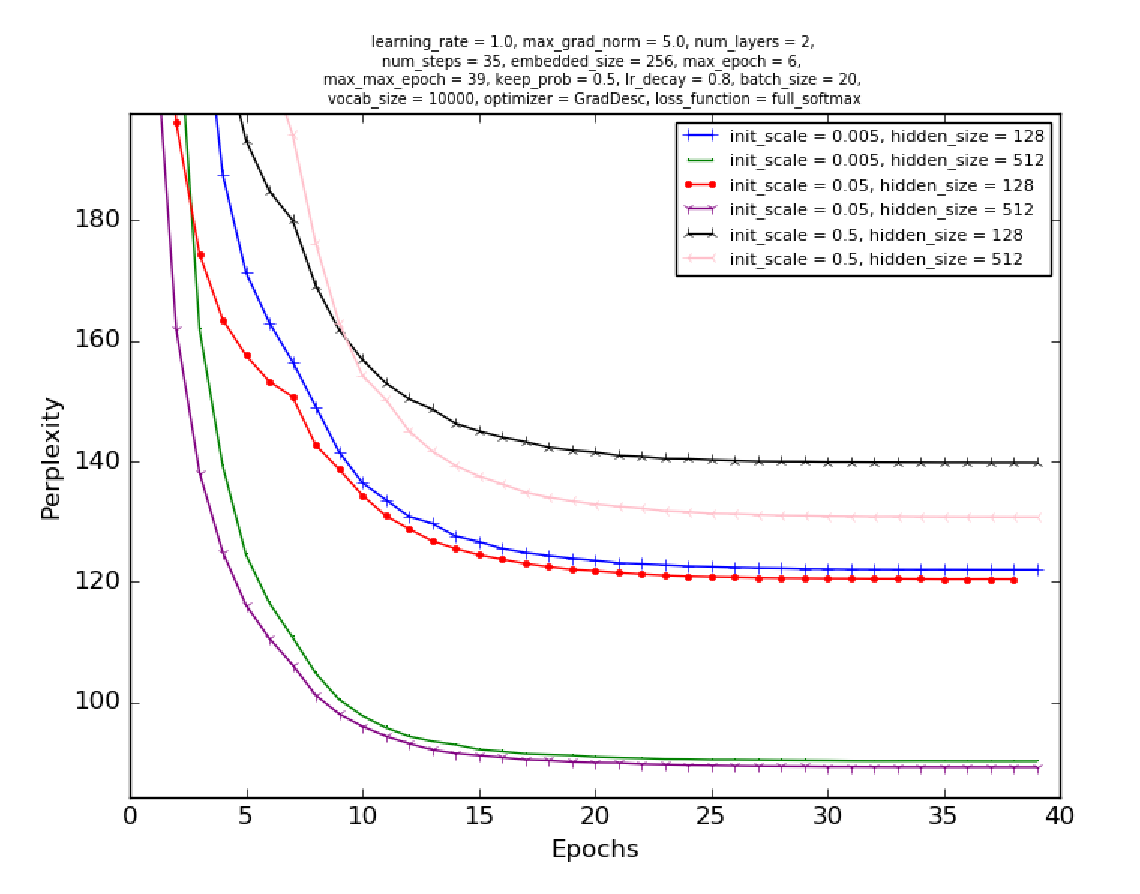
\includegraphics[width=0.80\textwidth]{Figures/inithiddenperf.eps}
		\caption{Convergence plot of the validation perplexity of the experiment with \textbf{init\_scale \& hidden\_size} as variable parameters. }
		\label{fig:exp2perf}
	\end{center}	
\end{figure}

The results of this experiment are displayed in table \ref{tab:exp2data} and figure \ref{fig:exp2perf}. In this case, bigger values for \textbf{hidden\_size} lead to better validation perplexities. 0.05 and 0.005 seem to be good values for \textbf{init\_scale}, while 0.5 leads to a significantly worse performance. This seems to imply that the weights of the network should be initialized at rather small values.\\
\\
The parameter \textbf{hidden\_size} naturally influences the training speed. As the value for this parameter goes up, the training slows down. \textbf{init\_scale} has no effect on the training speed.

\newpage

\subsection{hidden\_size \& embedded\_size}

\begin{table}[H]
\centering
\caption{Last training, validation and test perplexities and the training speed with \textbf{hidden\_size \& embedded\_size} as variable parameters.}
\label{tab:exp3data}
\begin{tabular}{|l|l|l|l|l|l|}
\hline
{\small Name} & {\small Train PPL} & {\small Valid PPL} & {\small Test PPL} & {\small Average speed}\\ \hline
{\small hidden\_size = 128, embedded\_size = 64  }       & 137.1526   & 129.8869   & 125.0642   & 11173.8044 \\ \hline
{\small hidden\_size = 128, embedded\_size = 128}        & 130.6858   & 125.0439   & 120.6486   & 11027.2286 \\ \hline
{\small hidden\_size = 128, embedded\_size = 256}        & 124.8371   & 120.8721   & 116.2822   & 11281.3936 \\ \hline
{\small hidden\_size = 256, embedded\_size = 64}         & 96.5572    & 106.1885   & 102.8703   & 8874.8156  \\ \hline
{\small hidden\_size = 256, embedded\_size = 128}        & 90.5044    & 101.9240   & 98.3112    & 8584.0692  \\ \hline
{\small hidden\_size = 256, embedded\_size = 256}        & 85.3554    & 98.3592    & 94.8026    & 8698.9466  \\ \hline
{\small hidden\_size = 512, embedded\_size = 64}         & 66.7117    & 94.9333    & 92.1504    & 5268.9036  \\ \hline
{\small hidden\_size = 512, embedded\_size = 128}        & 60.8136    & 91.5243    & 87.9890    & 5461.2367  \\ \hline
{\small hidden\_size = 512, embedded\_size = 256}        & 56.8551    & 89.6501    & 86.0614    & 5311.4149  \\ \hline
\end{tabular}
\end{table}

\begin{figure}[H]
	\begin{center}
		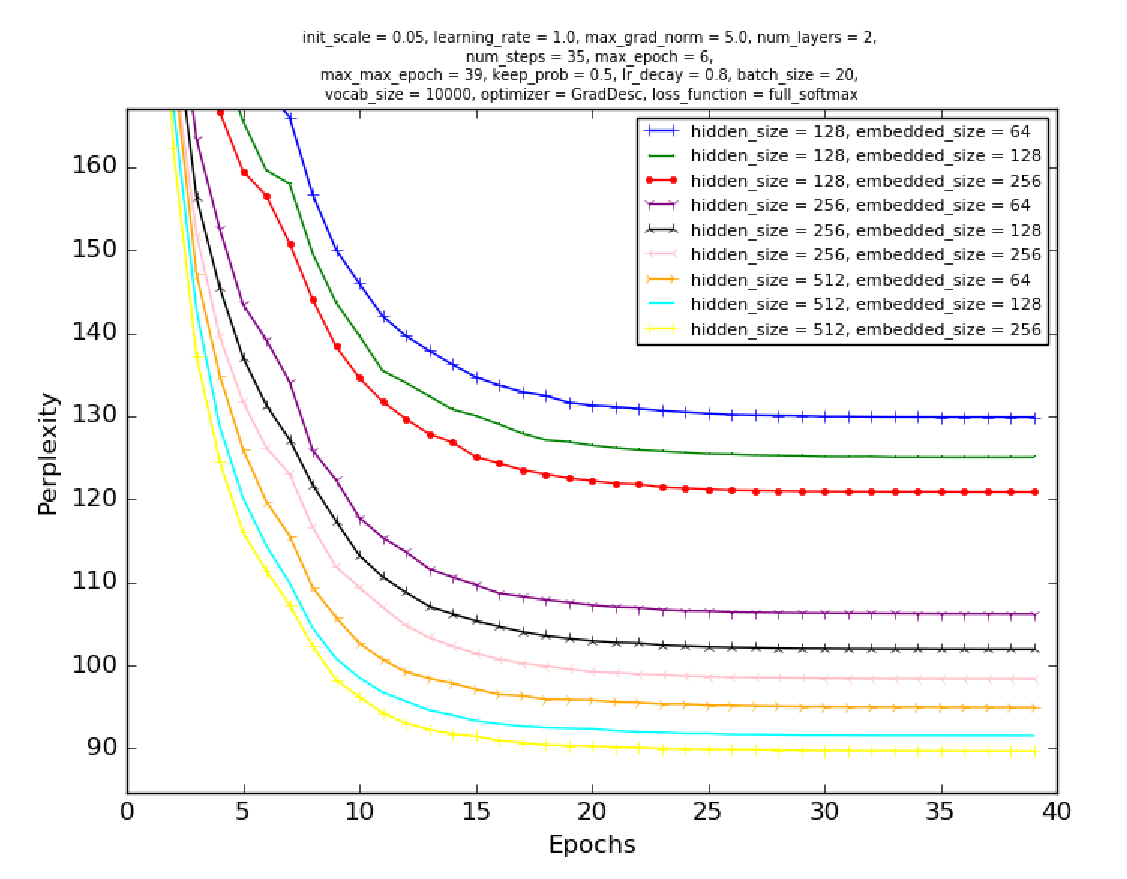
\includegraphics[width=0.80\textwidth]{Figures/hiddenembeddedperf.eps}
		\caption{Convergence plot of the validation perplexity of the experiment with \textbf{hidden\_size \& embedded\_size} as variable parameters.}
		\label{fig:exp3perf}
	\end{center}	
\end{figure}

The results of this experiment are displayed in table \ref{tab:exp3data} and figure \ref{fig:exp3perf}. The results are mostly as expected: higher values for \textbf{hidden\_size} generally lead to better performance and slower training speed and higher values for \textbf{embedded\_size} lead to better performance (though less impactful than \textbf{hidden\_size}). However, the parameter \textbf{embedded\_size} does not seem to have a big impact (if any at all) on the training speed. This is interesting as it might suggest that increasing \textbf{embedded\_size} only has positive consequences (at least while the parameter is kept within a certain range).
\newpage

\subsection{max\_grad\_norm}

\begin{table}[H]
\centering
\caption{Last training, validation and test perplexities and the training speed with \textbf{max\_grad\_norm} as variable parameter.}
\label{tab:exp4data}
\begin{tabular}{|l|l|l|l|l|l|}
\hline
{\small Name} & {\small Train PPL} & {\small Valid PPL} & {\small Test PPL} & {\small Average speed}\\ \hline
{\small max\_grad\_norm = 1.0}                           & 103.9493   & 120.8001   & 118.1674   & 5322.4864  \\ \hline
{\small max\_grad\_norm = 5.0 }                          & 56.8391    & 89.2325    & 85.9046    & 5309.6957  \\ \hline
{\small max\_grad\_norm = 10.0 }                         & 61.9130    & 90.0071    & 86.5227    & 5328.3798  \\ \hline
\end{tabular}
\end{table}

\begin{figure}[H]
	\begin{center}
		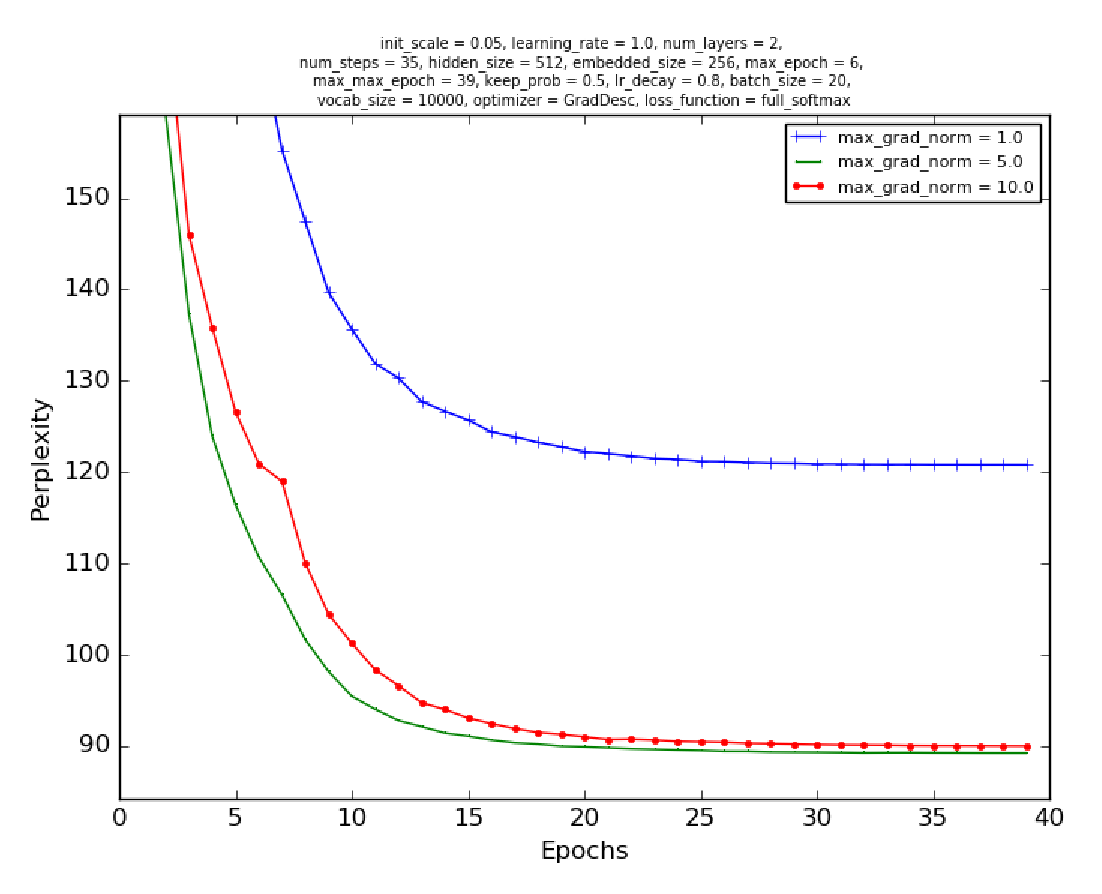
\includegraphics[width=0.80\textwidth]{Figures/maxgradperf.eps}
		\caption{Convergence plot of the validation perplexity of the experiment with \textbf{max\_grad\_norm} as variable parameter. }
		\label{fig:exp4perf}
	\end{center}	
\end{figure}

The results of this experiment are displayed in table \ref{tab:exp4data} and figure \ref{fig:exp4perf}. Choosing \textbf{max\_grad\_norm} equal to 1 is clearly not a good idea: the clipping of the gradients is too strong and the changes to the weights of the network are too small. This leads to a bad validation perplexity. For the other two cases, there does not seem to be much difference in performance.\\
\\
This parameter has no impact on the training speed.

\newpage

\subsection{num\_layers}

\begin{table}[H]
\centering
\caption{Last training, validation and test perplexities and the training speed with \textbf{num\_layers} as variable parameter.}
\label{tab:exp5data}
\begin{tabular}{|l|l|l|l|l|l|}
\hline
{\small Name} & {\small Train PPL} & {\small Valid PPL} & {\small Test PPL} & {\small Average speed}\\ \hline
{\small num\_layers = 1 }                               & 52.6574    & 87.7519    & 84.3744    & 8781.3653  \\ \hline
{\small num\_layers = 2}                                & 56.4768    & 88.8830    & 85.7698    & 5318.5357  \\ \hline
{\small num\_layers = 3}                                & 61.5084    & 93.3361    & 90.2382    & 3842.1562  \\ \hline
\end{tabular}
\end{table}

\begin{figure}[H]
	\begin{center}
		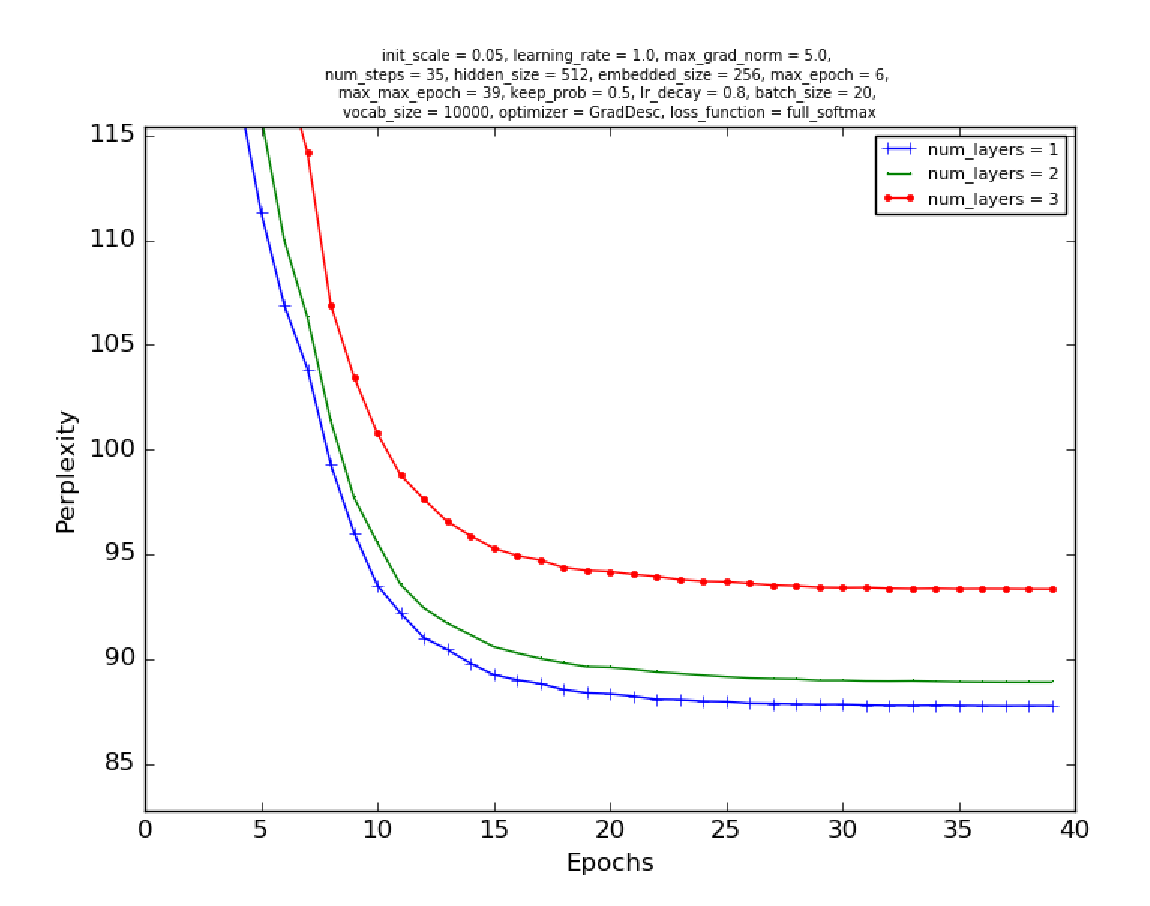
\includegraphics[width=0.80\textwidth]{Figures/numlayersperf.eps}
		\caption{Convergence plot of the validation perplexity of the experiment with \textbf{num\_layers} as variable parameter. }
		\label{fig:exp5perf}
	\end{center}	
\end{figure}

The results of this experiment are displayed in table \ref{tab:exp5data} and figure \ref{fig:exp5perf}. The results seem to indicate that in this case it is better to stay away from multiple layers of LSTM cells. This could be because the number of model parameters (weights) increase heavily as \textbf{num\_layers} is increased, and there might not be enough training data available to cope with huge amounts of parameters.\\
\\
As expected, the training speed goes down significantly when the number of layers is increased. 

\newpage

\subsection{num\_steps \& batch\_size}

\begin{table}[H]
\centering
\caption{Last training, validation and test perplexities and the training speed with \textbf{num\_steps \& batch\_size} as variable parameters.}
\label{tab:exp6data}
\begin{tabular}{|l|l|l|l|l|l|}
\hline
{\small Name} & {\small Train PPL} & {\small Valid PPL} & {\small Test PPL} & {\small Average speed}\\ \hline
{\small num\_steps = 20, batch\_size = 10}               & 63.8183    & 91.3286    & 87.3871    & 2841.4514  \\ \hline
{\small num\_steps = 35, batch\_size = 10}               & 57.4925    & 87.9364    & 84.7437    & 2967.6752  \\ \hline
{\small num\_steps = 50, batch\_size = 10}               & 55.6267    & 87.5726    & 84.1104    & 3032.4830  \\ \hline
{\small num\_steps = 20, batch\_size = 20}               & 57.7876    & 89.4243    & 85.4032    & 5283.1615  \\ \hline
{\small num\_steps = 35, batch\_size = 20}               & 56.8357    & 89.0865    & 86.1965    & 5327.4472  \\ \hline
{\small num\_steps = 50, batch\_size = 20}               & 57.4257    & 89.8376    & 86.9127    & 5340.5170  \\ \hline
{\small num\_steps = 20, batch\_size = 40}               & 58.0128    & 91.2085    & 87.4406    & 7340.3399  \\ \hline
{\small num\_steps = 35, batch\_size = 40}               & 59.9359    & 92.4088    & 89.0932    & 7222.8050  \\ \hline
{\small num\_steps = 50, batch\_size = 40}               & 63.9817    & 95.3053    & 91.6211    & 7685.0879  \\ \hline
\end{tabular}
\end{table}

\begin{figure}[H]
	\begin{center}
		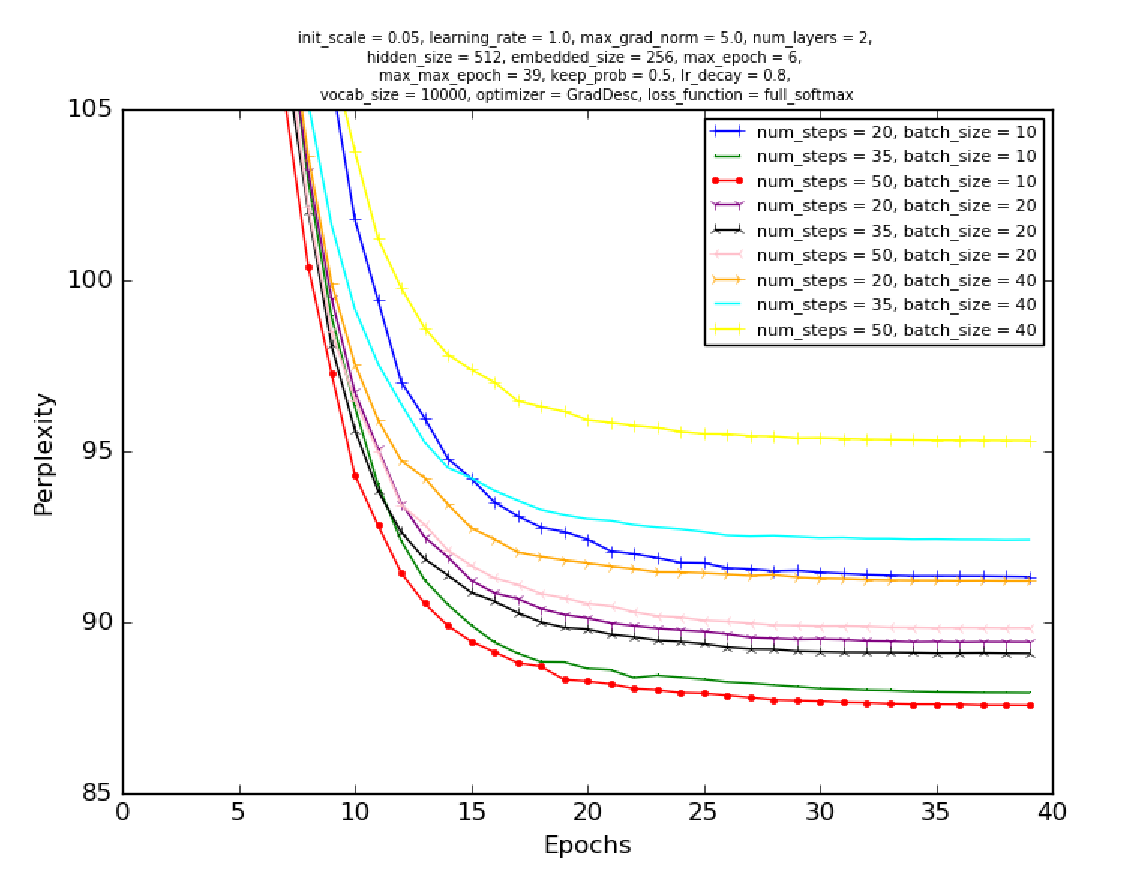
\includegraphics[width=0.80\textwidth]{Figures/numstepsbatchperf.eps}
		\caption{Convergence plot of the validation perplexity of the experiment with \textbf{num\_steps \& batch\_size} as variable parameters. }
		\label{fig:exp6perf}
	\end{center}	
\end{figure}

The results of this experiment are displayed in table \ref{tab:exp6data} and figure \ref{fig:exp6perf}. As expected,  as \textbf{batch\_size} goes up, the training speed slows down while there seems to be very little impact of \textbf{num\_steps} on the training speed. When it comes to the performance the results are not very clear: there seem to be local optima for these parameters. No definitive conclusion can be made based on this experiment.

\newpage

\subsection{num\_steps}

\begin{table}[H]
\centering
\caption{Last training, validation and test perplexities and the training speed with \textbf{num\_steps} as variable parameter.}
\label{tab:exp7data}
\begin{tabular}{|l|l|l|l|l|l|}
\hline
{\small Name} & {\small Train PPL} & {\small Valid PPL} & {\small Test PPL} & {\small Average speed}\\ \hline
{\small num\_steps = 15}                                & 59.9904    & 89.7558    & 86.1790    & 4796.6922  \\ \hline
{\small num\_steps = 35}                                & 56.3721    & 88.4145    & 85.7701    & 5317.4104  \\ \hline
{\small num\_steps = 55}                                & 58.1670    & 91.1254    & 87.9059    & 5522.2976  \\ \hline
{\small num\_steps = 75}                                & 60.4014    & 92.5607    & 89.4328    & 5606.5938  \\ \hline
\end{tabular}
\end{table}

\begin{figure}[H]
	\begin{center}
		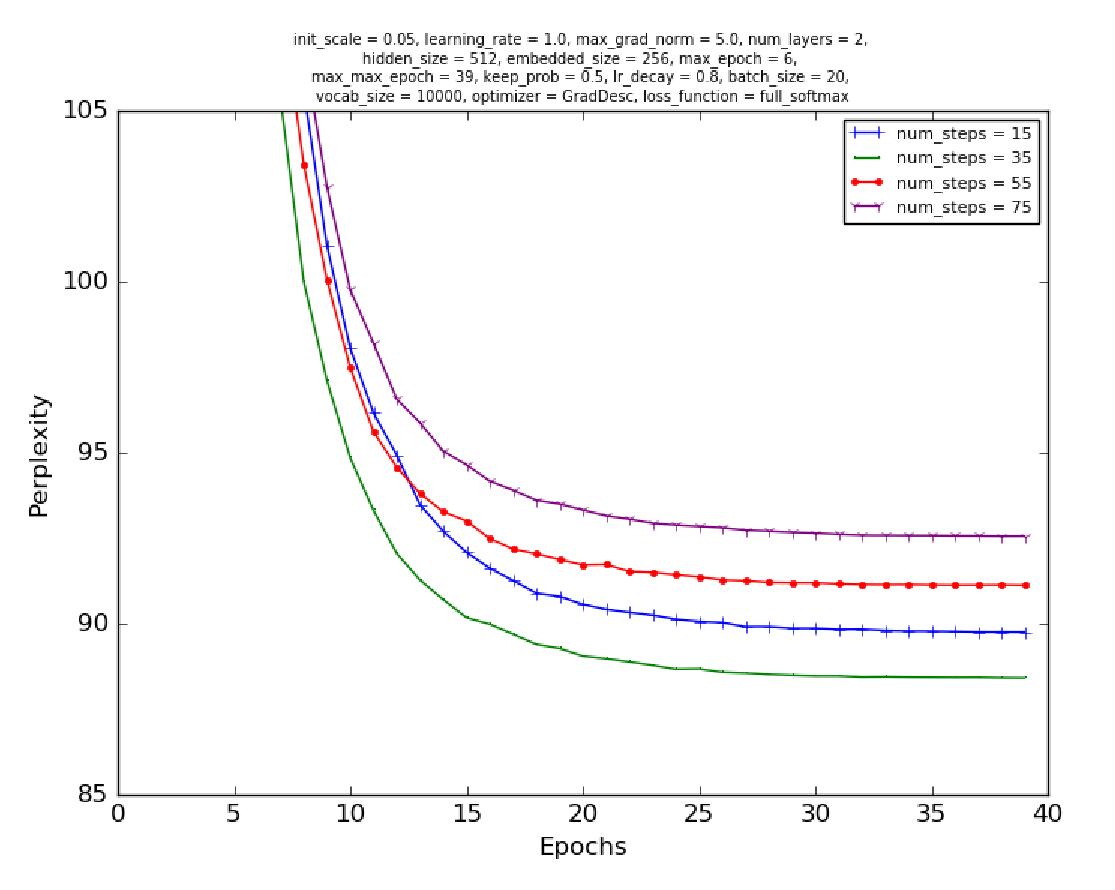
\includegraphics[width=0.80\textwidth]{Figures/numstepsperf.eps}
		\caption{Convergence plot of the validation perplexity of the experiment with \textbf{num\_steps} as variable parameter. }
		\label{fig:exp7perf}
	\end{center}	
\end{figure}

The results of this experiment are displayed in table \ref{tab:exp7data} and figure \ref{fig:exp7perf}. The figure shows a local optimum for \textbf{num\_steps} equal to 35. This is somewhat strange as one would expect the performance to go up when more time steps are taken into account for training.\\
\\
The training speed seems to go down as \textbf{num\_steps} is reduced, which is logical as each element of the training batch has length \textbf{num\_steps}. This leads to less batches in one epoch, hence there are less weight updates per epoch and the speed goes up.

\newpage

\subsection{optimizer}

\begin{table}[H]
\centering
\caption{Last training, validation and test perplexities and the training speed with \textbf{optimizer} as variable parameter.}
\label{tab:exp8data}
\begin{tabular}{|l|l|l|l|l|l|}
\hline
{\small Name} & {\small Train PPL} & {\small Valid PPL} & {\small Test PPL} & {\small Average speed}\\ \hline
optimizer = GradDesc                          & 56.5491    & 89.0828    & 85.6273    & 5324.8581  \\ \hline
optimizer = Adadelta                          & 764.3933   & 720.4745   & 689.8613   & 5188.6086  \\ \hline
optimizer = Adagrad                           & 67.8530    & 97.5119    & 93.7309    & 5261.3310  \\ \hline
optimizer = Adam                              & 66.7381    & 118.1673   & 108.4468   & 4806.0537  \\ \hline
optimizer = Momentum                          & 58.1349    & 88.0675    & 84.2937    & 5264.8214  \\ \hline
\end{tabular}
\end{table}

\begin{figure}[H]
	\begin{center}
		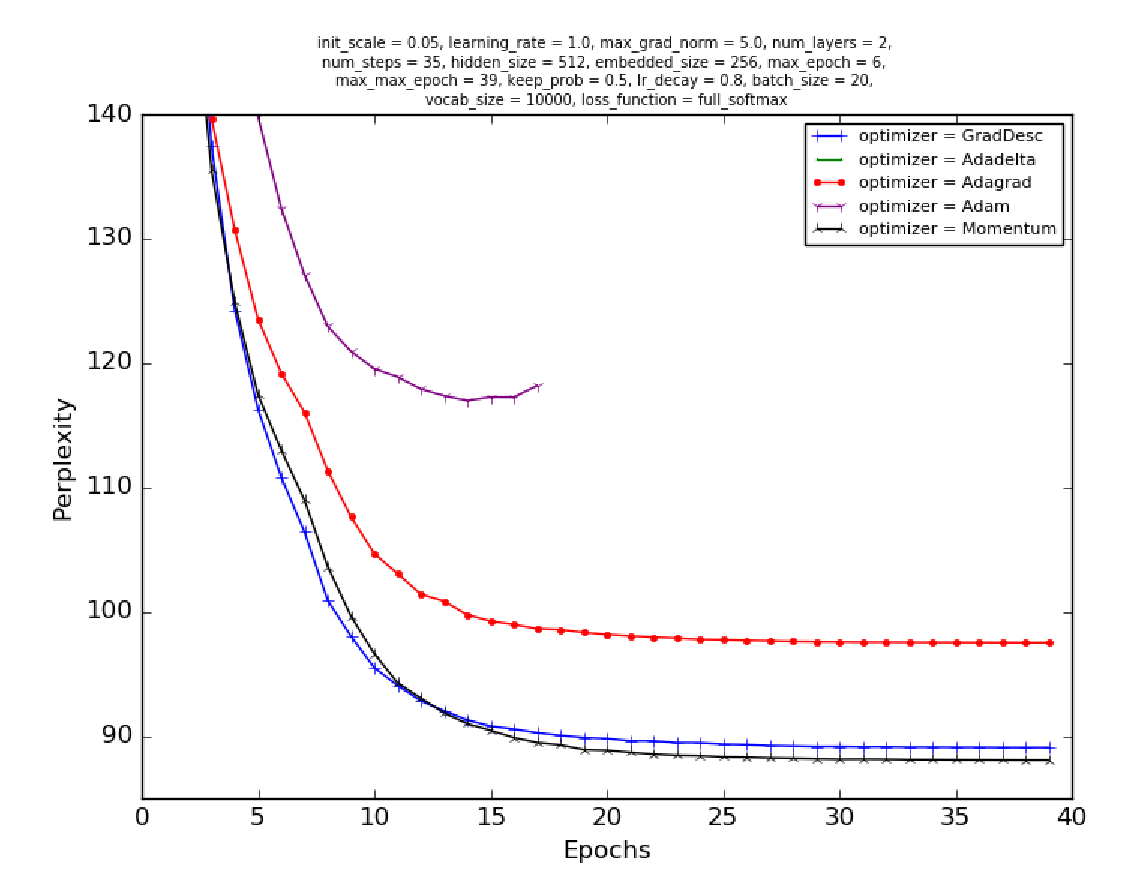
\includegraphics[width=0.80\textwidth]{Figures/optimizerperf.eps}
		\caption{Convergence plot of the validation perplexity of the experiment with \textbf{optimizer} as variable parameter. The Adagrad optimizer is not shown because his last perplexity at epoch 39 was still far above the others.}
		\label{fig:exp8perf}
	\end{center}	
\end{figure}

The results of this experiment are displayed in table \ref{tab:exp8data} and figure \ref{fig:exp8perf}. There seems be one big loser in this experiment: the Adadelta optimizing algorithm. Adam also doesn't seem to perform well and is also the slowest. Adagrad is slightly better, but the gradient descent and momentum algorithms are the clear winners of this experiment. 

\newpage

\subsection{loss\_function}

\begin{table}[H]
\centering
\caption{Last training, validation and test perplexities and the training speed with \textbf{loss\_function} as variable parameter.}
\label{tab:exp9data}
\begin{tabular}{|l|l|l|l|l|l|}
\hline
{\small Name} & {\small Train PPL} & {\small Valid PPL} & {\small Test PPL} & {\small Average speed}\\ \hline
{\small loss\_function = full softmax }                 & 56.7543    & 88.6126    & 85.5887    & 5318.9263  \\ \hline
{\small loss\_function = sampled softmax }              & 4.7374     & 99.3000    & 94.9911    & 6250.8133  \\ \hline
\end{tabular}
\end{table}

\begin{figure}[H]
	\begin{center}
		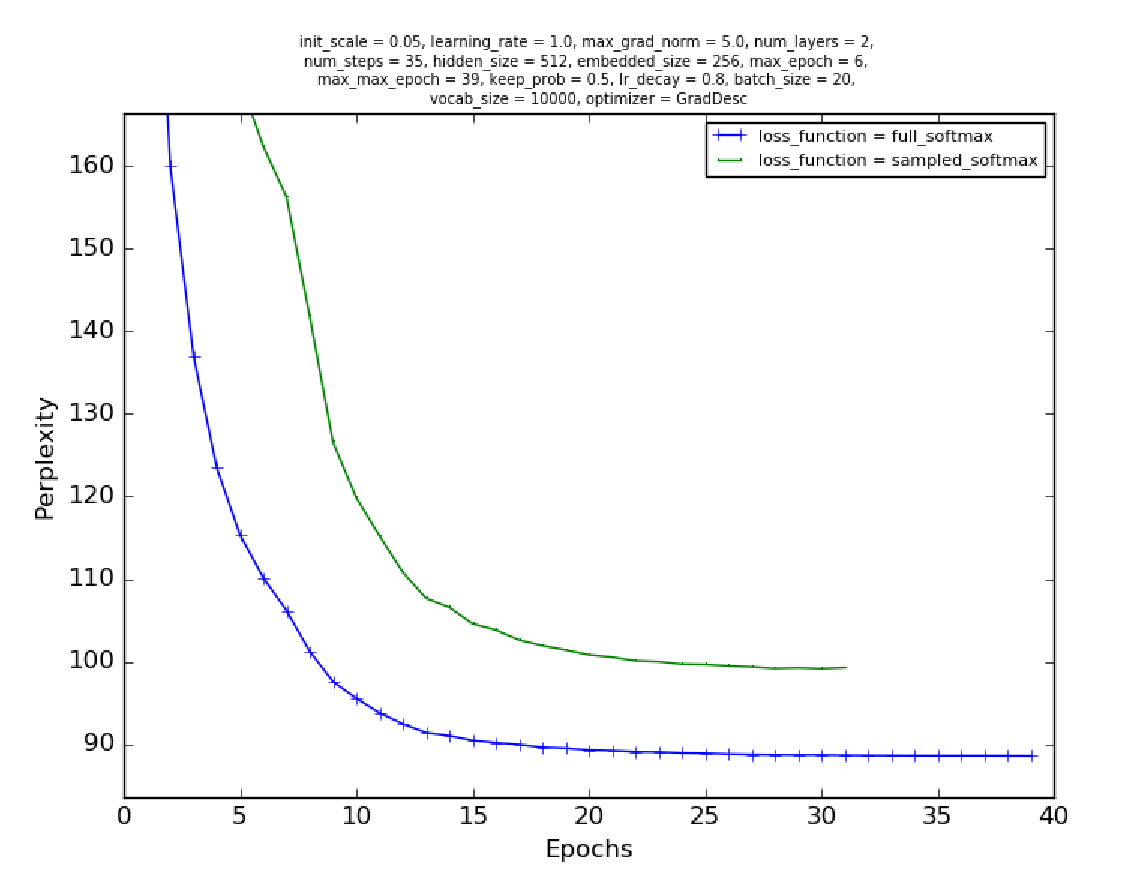
\includegraphics[width=0.80\textwidth]{Figures/lossperf.eps}
		\caption{Convergence plot of the validation perplexity of the experiment with \textbf{loss\_function} as variable parameter. }
		\label{fig:exp9perf}
	\end{center}	
\end{figure}

The results of this experiment are displayed in table \ref{tab:exp9data} and figure \ref{fig:exp9perf}. The results are as expected, the sampled softmax loss function trains quicker but performs worse than the full softmax function. Extra experiments will have to be done to see if this loss in performance is worth the gain in speed.\\
\\
Please note that the training perplexity when using the sampled softmax loss function is not a real perplexity value. This is because the training perplexity is calculated based on the output of the sampled softmax probablities. These probabilities are not properly normalized, as described in section \ref{subsubsec:loss}, and hence the training performance is strongly overestimated.

\newpage

\section{Conclusion}

These experiments investigated the impact of the different training parameters involved when using recurrent neural networks for language modeling. To this end, the TensorFlow tutorial model of a recurrent neural network for language modeling (publicly available) was used with the Penn TreeBank dataset for training, validation and testing of the model \cite{tensorflow}.\\
\\
The most interesting conclusions that could be drawn from these experiments are summarized in this list (see section \ref{subsec:exp} for an explanation of the parameters):

\begin{itemize}
	\item Increasing \textbf{hidden\_size} improves performance but lowers training speed.
	\item Increasing \textbf{embedded\_size} improves performance slightly but does not have an impact or very little impact on training speed.
	\item \textbf{init\_scale} should be kept at a relatively low value.	
	\item \textbf{learning\_rate} should be kept at a relatively high value and \textbf{lr\_decay} should not be too high.
	\item \textbf{max\_grad\_norm} should not be too low as this hinders the learning process of the network.
	\item Increasing \textbf{num\_steps} makes training faster, regarding performance this parameter seems to have a local optimum. 
	\item The sampled softmax loss function has worse performance but better training speed than the full softmax loss function. 
	\item The gradient descent and momentum optimization algorithms do better than the other algorithms in terms of performance and speed.
	\item The optimal value for \textbf{num\_layers} in this case is 1. However, this could be because there is not enough training data to properly train the model when multiple LSTM layers are employed.
\end{itemize}


\newpage
\addcontentsline{toc}{section}{References}
\begin{thebibliography}{9}
	
	\bibitem{tensorflow}
	\textit{https://www.tensorflow.org/versions/r0.11/tutorials/recurrent/index.html}
	
	\bibitem{LSTM}
	\textit{http://colah.github.io/posts/2015-08-Understanding-LSTMs/}
	
	\bibitem{PTB}
	\textit{http://www.cis.upenn.edu/~treebank/home.html}
	
	\bibitem{dropout}
	\textit{https://www.cs.toronto.edu/~hinton/absps/JMLRdropout.pdf}
	
	\bibitem{opt}
	\textit{https://www.tensorflow.org/versions/r0.11/api\_docs/python/train.html}
	
	\bibitem{bptt}
	\textit{http://ir.hit.edu.cn/~jguo/docs/notes/bptt.pdf}
	
	\bibitem{exp}
	\textit{http://www.wildml.com/2015/10/recurrent-neural-networks-tutorial-part-3-backpropagation-through-time-and-vanishing-gradients/}
	
	\bibitem{cross}
	\textit{http://homes.esat.kuleuven.be/~jpeleman/wim\_en\_robbe/jurafsky04.pdf}
	
	\bibitem{sampled}
	\textit{https://arxiv.org/pdf/1412.2007v2.pdf}
	
\end{thebibliography}
	
\end{document}